\textit{Phenomenological models} represent simple and abstract models of synapses, which are
computationally light and optimal from a functional point of view (synaptic current computation), though not reliable
from a biological one. On the opposite, \textit{biophysical models} are focused on the modelling
of the biochemical processes involved in the synaptic transmission.\\
There are two types of synaptic transmission:
\begin{itemize}
    \item \textbf{Electrical}: this method of signal propagation is extremely
          fast and it is employed by cortex interneurons.
    \item \textbf{Chemical}: this is the most common way for neural signal
          to travel, even if it is a bit slower.
\end{itemize}

\subsection{Electrical Synaptic Transmission}
Before designing a model, it is compulsory understanding how a biological system
actually works. In electrical synapses, the ions flow through the connexons,
which can be regarded as channels. Note that there is no synaptic cleft in
the case of electrical transmission. The propagation speed of the signal is
thus extremely fast.
\begin{figure}[H]
    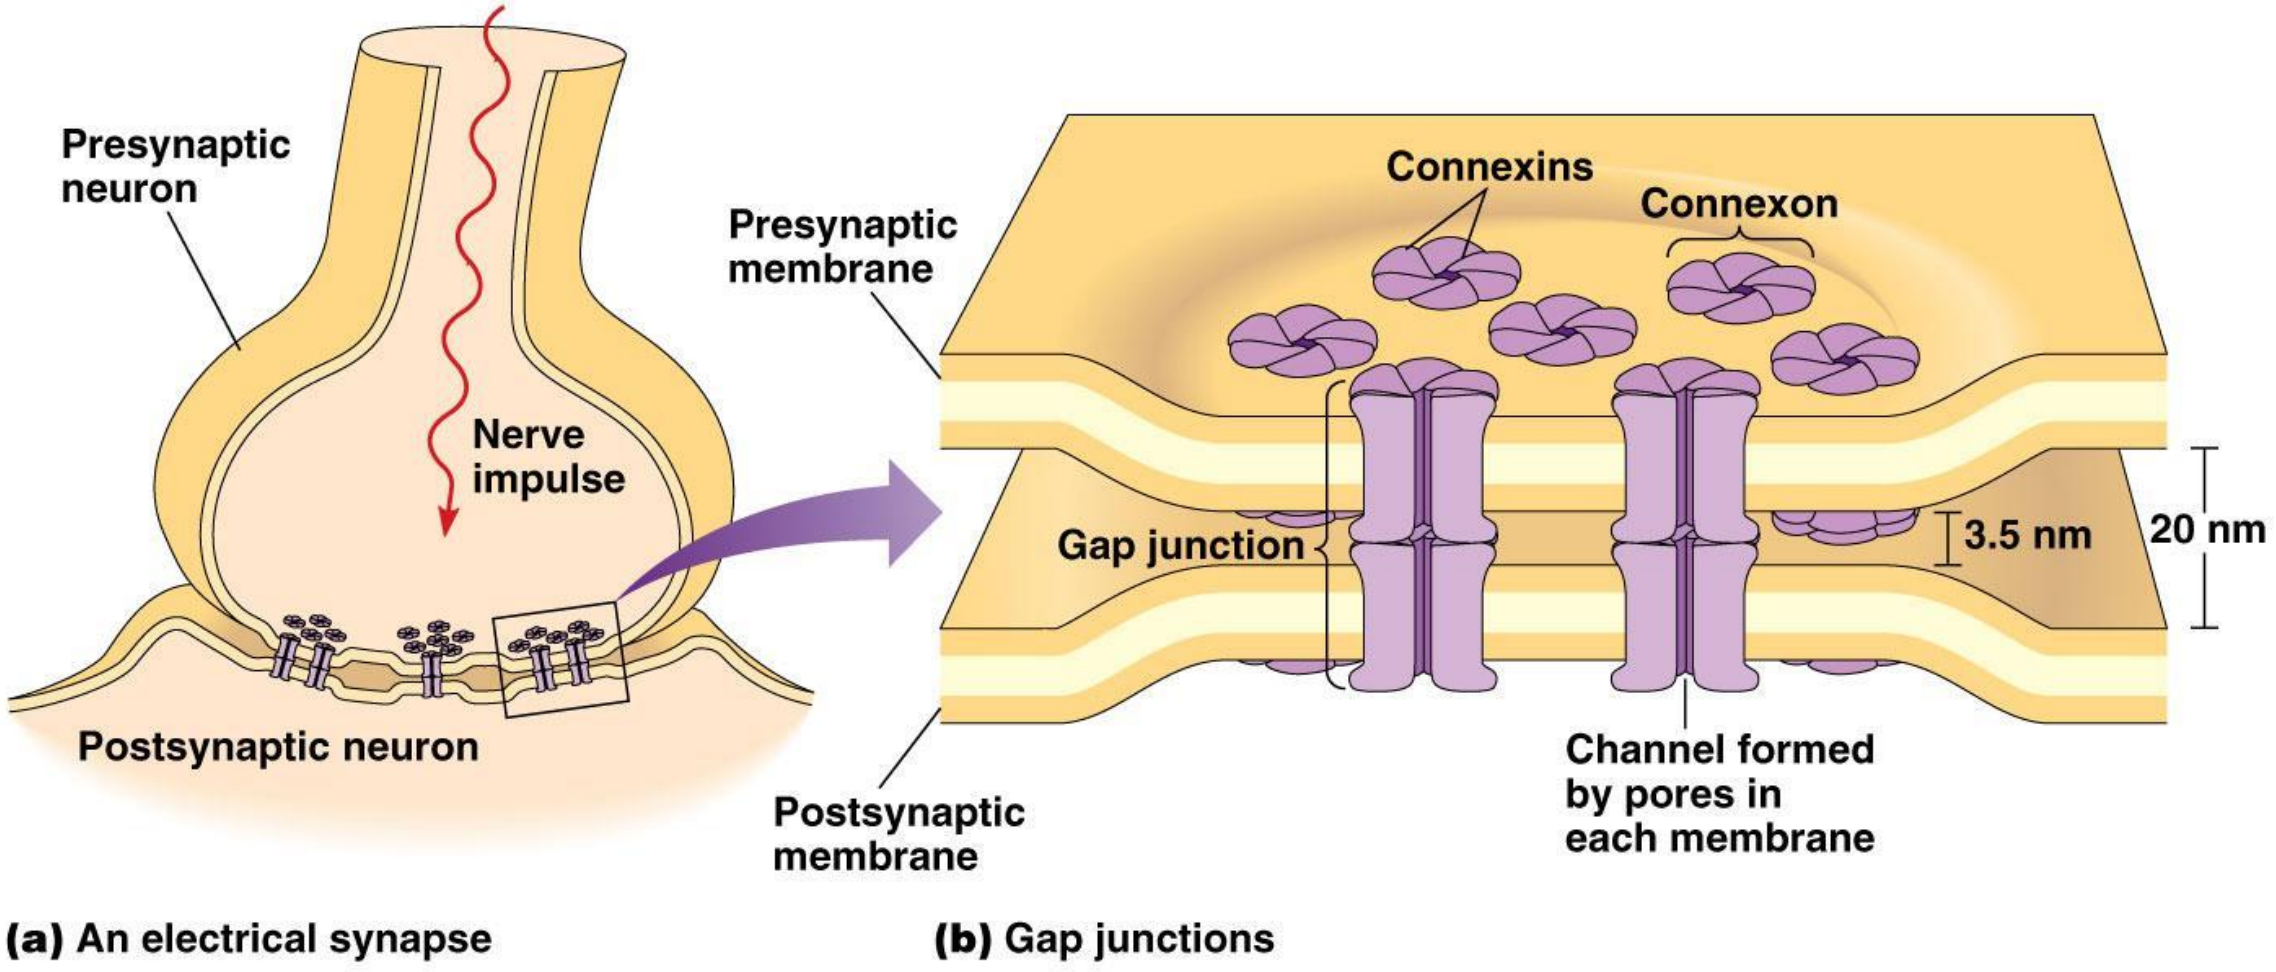
\includegraphics[scale=0.32]{12_1}
    \centering
\end{figure}
The electrical synapse electrophysiological features are:
\begin{itemize}
    \item \textbf{Bidirectionality}: the direction of signal propagation is
          not unique, as pre and post synaptic neurons are alike.
    \item \textbf{Speed}: the propagation speed is considerably high.
    \item \textbf{Absence of a Sign}: inhibitory and excitatory synapses
          cannot be distinguished, as the effect is determined by the direction of
          the electrical current.
\end{itemize}
To model a single gap junction it is sufficient to employ a conductance behaving as
a constant resistor, which represents the electrical coupling between the
two communicating neurons:
\begin{equation*}
    I_{syn}=g_{gap}\cdot{(V_{pre}-V_{post})}
\end{equation*}
Note that in this case no plasticity nor second messengers are involved.\\
Let's now analyse what happens when multiple neurons are connected one after another
and how the signal propagates. This can be done by introducing the Transfer-Impedance
\(Z_{ab}\) between two electrically coupled cells \(a\) and \(b\). It is computed as
the ratio of Fourier transforms of the voltage responses \(V_{a}\) and \(V_{b}\)
recorded simultaneously upon the injection of a current in one of the two cells.
Note that the smallest number of intermediate cells connecting electrically two neurons
coincides with the high frequency power law exponent of the Transfer-Impedance:
\begin{equation*}
    Z_{ab}\sim{(j\omega)^{-d}}
\end{equation*}
where \(d\) is the proximity or distance.\\
Therefore, the proximity of electrical coupling is inferred from the slope of Transfer-Impedance.
Note that such an approach works only for electrical synapses, displaying a constant (time-invariant)
conductance.
\begin{figure}[H]
    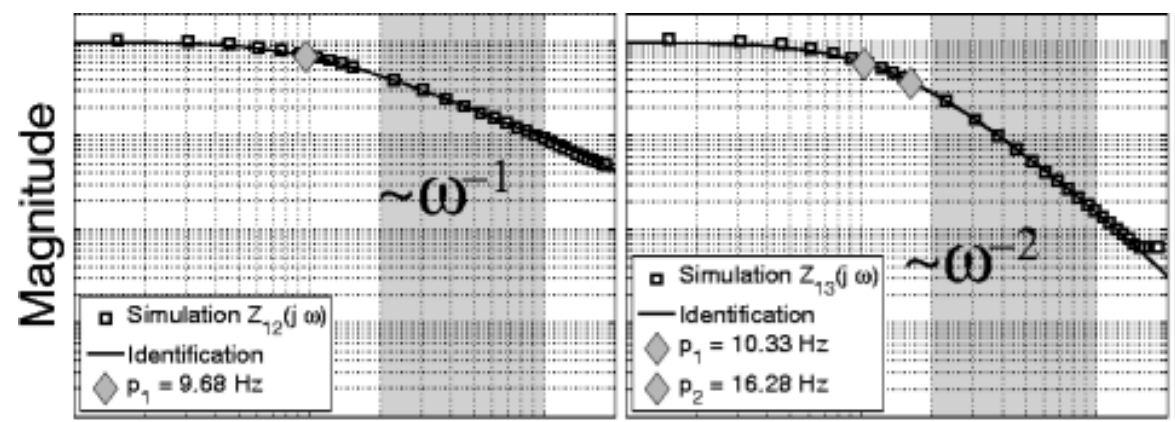
\includegraphics[scale=0.5]{12_2}
    \centering
\end{figure}
Note that this approach allows to estimate the number of interneurons between the stimulated
cell and the recorded one.

\subsection{Chemical Synaptic Transmission}
Nowadays, most of the research about synapses is focused on understanding and modelling
chemical synapses, as they are widely spread and more complex than the electrical ones.
\begin{figure}[H]
    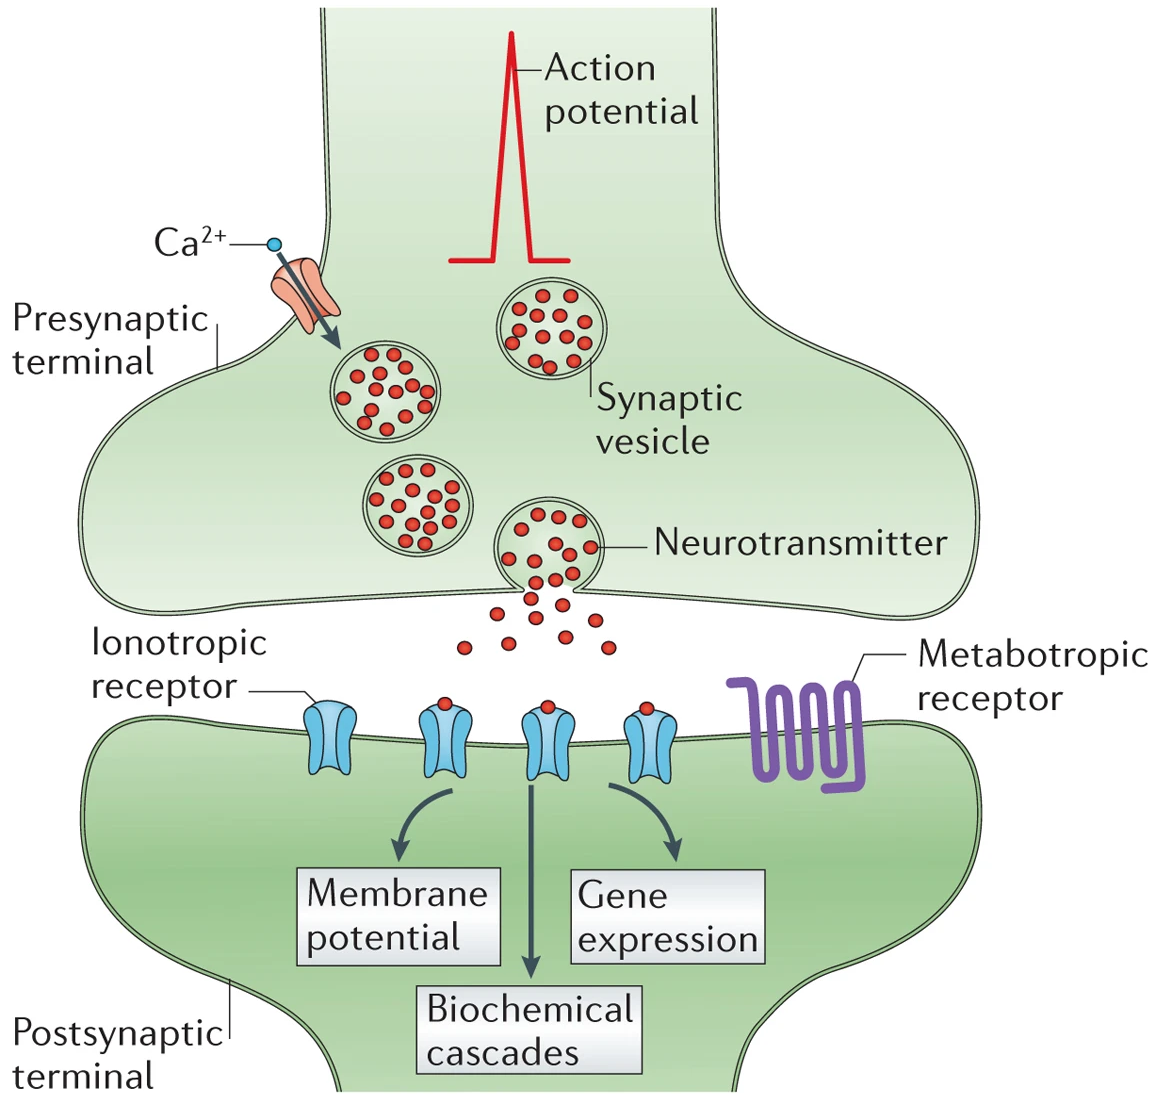
\includegraphics[scale=0.28]{12_3}
    \centering
\end{figure}
In chemical synapses, pre and post synaptic terminals are well distinguished, as they
require different morphological structures: as a consequence they are to be
modelled differently. Moreover, a synaptic cleft of approximately \(20\,nm\) is present.\\
When the goal is building a chemical synapse model, it is crucial to decide which
components of the involved biochemical reactions are to be considered. The classical
chemical neurotransmission follows these steps:
\begin{enumerate}
    \item Neurotransmitters sit inside synaptic vescicles in the presynaptic terminal.
    \item An incoming action potential propagates through the neuron and causes an influx
    of Ca\({}^{2+}\) ions via voltage-gated calcium channels.
    \item The vescicles move toward the membrane and they fuse with it and the neurotransmitters
    are released in the synaptic cleft.
    \item Neurotransmitters diffuse across the synaptic cleft and bind to the receptors of
    the postsynaptic cell.
    \item The postsynaptic cell opens its ionic channels, allowing the change of the membrane potential,
    eventually eliciting an action potential.
\end{enumerate}
It is fundamental to state that each neurotransmitter is associated to specific receptors at the
postsynaptic level. Therefore, the presynaptic neuron can always be modelled in the same way,
while the postsynaptic one will change according to the considered kinds of receptors, each one
with its own kinetics.\\
Two distinct types of neurotransmission exist:
\begin{itemize}
    \item \textbf{Ionotropic Neurotransmission}: the neurotransmitter reacts with the channel and its
    gate passes to the open state. This mechanism is \textit{fast}.
    \item \textbf{Metabotropic Neurotransmission}: the neurotransmitter reacts with second messengers
    receptors, which release second messengers inside the cells, which then open the ionic channels.
    This mechanism has a \textit{slow} onset, but might last much longer.
\end{itemize}
In addition, note that neurotransmitters can be either \textbf{excitatory} or \textbf{inhibitory}.
\begin{figure}[H]
    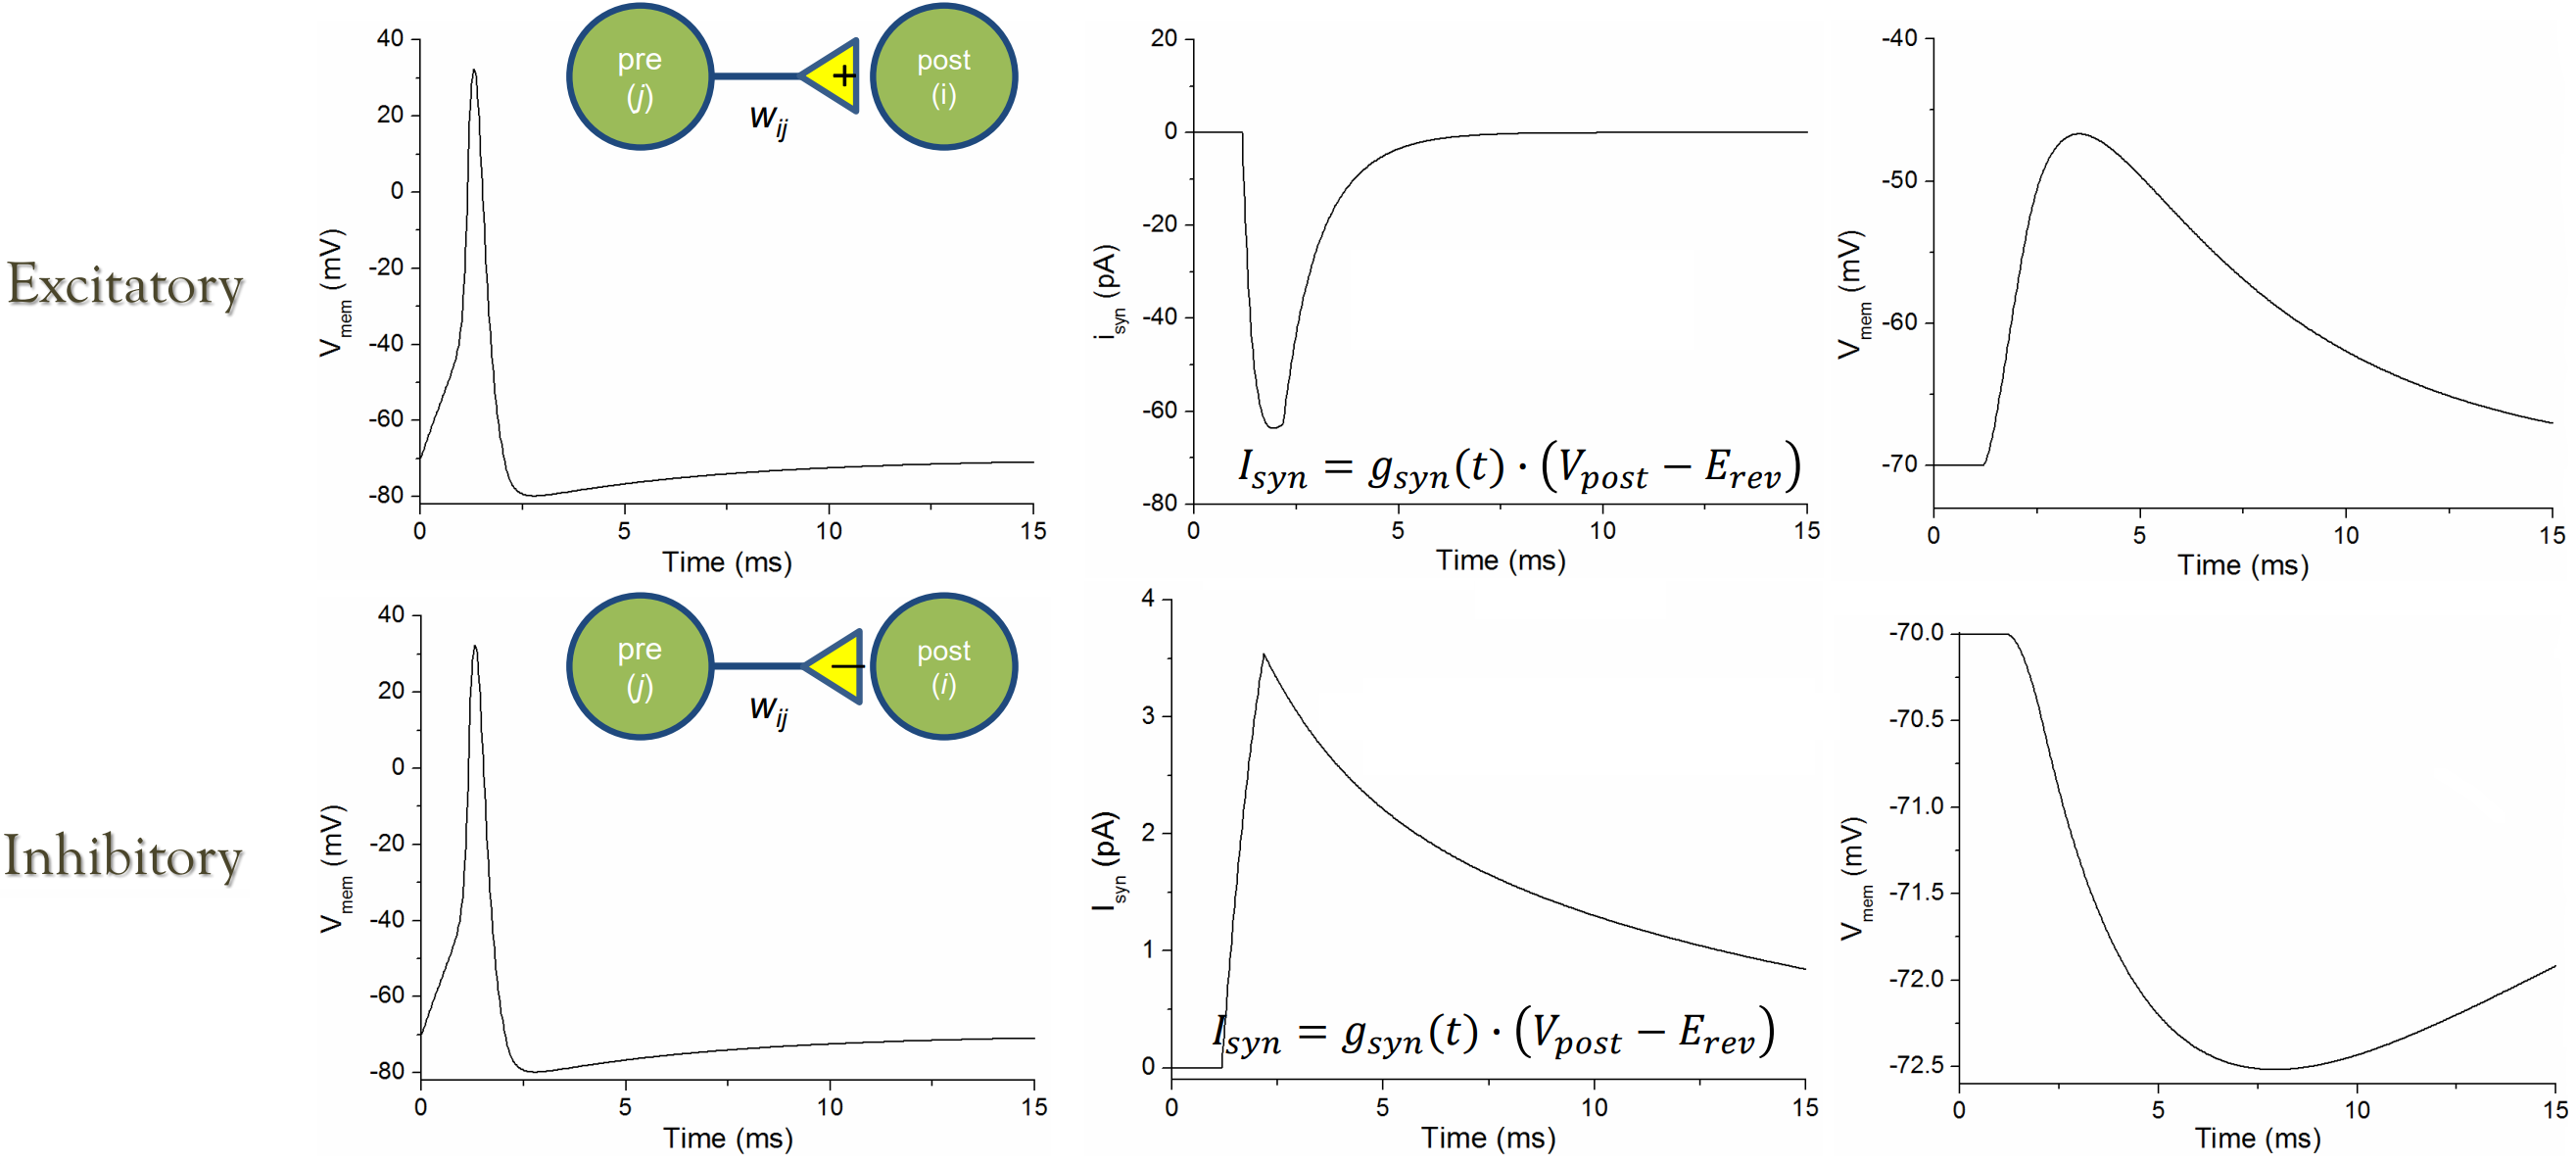
\includegraphics[scale=0.29]{12_4}
    \centering
\end{figure}
Another crucial property of synapses is that the effect of the depolarizations or
hyperpolarizations in the postsynaptic cell are integrated both from spatial and
temporal viewpoints.
\begin{figure}[H]
    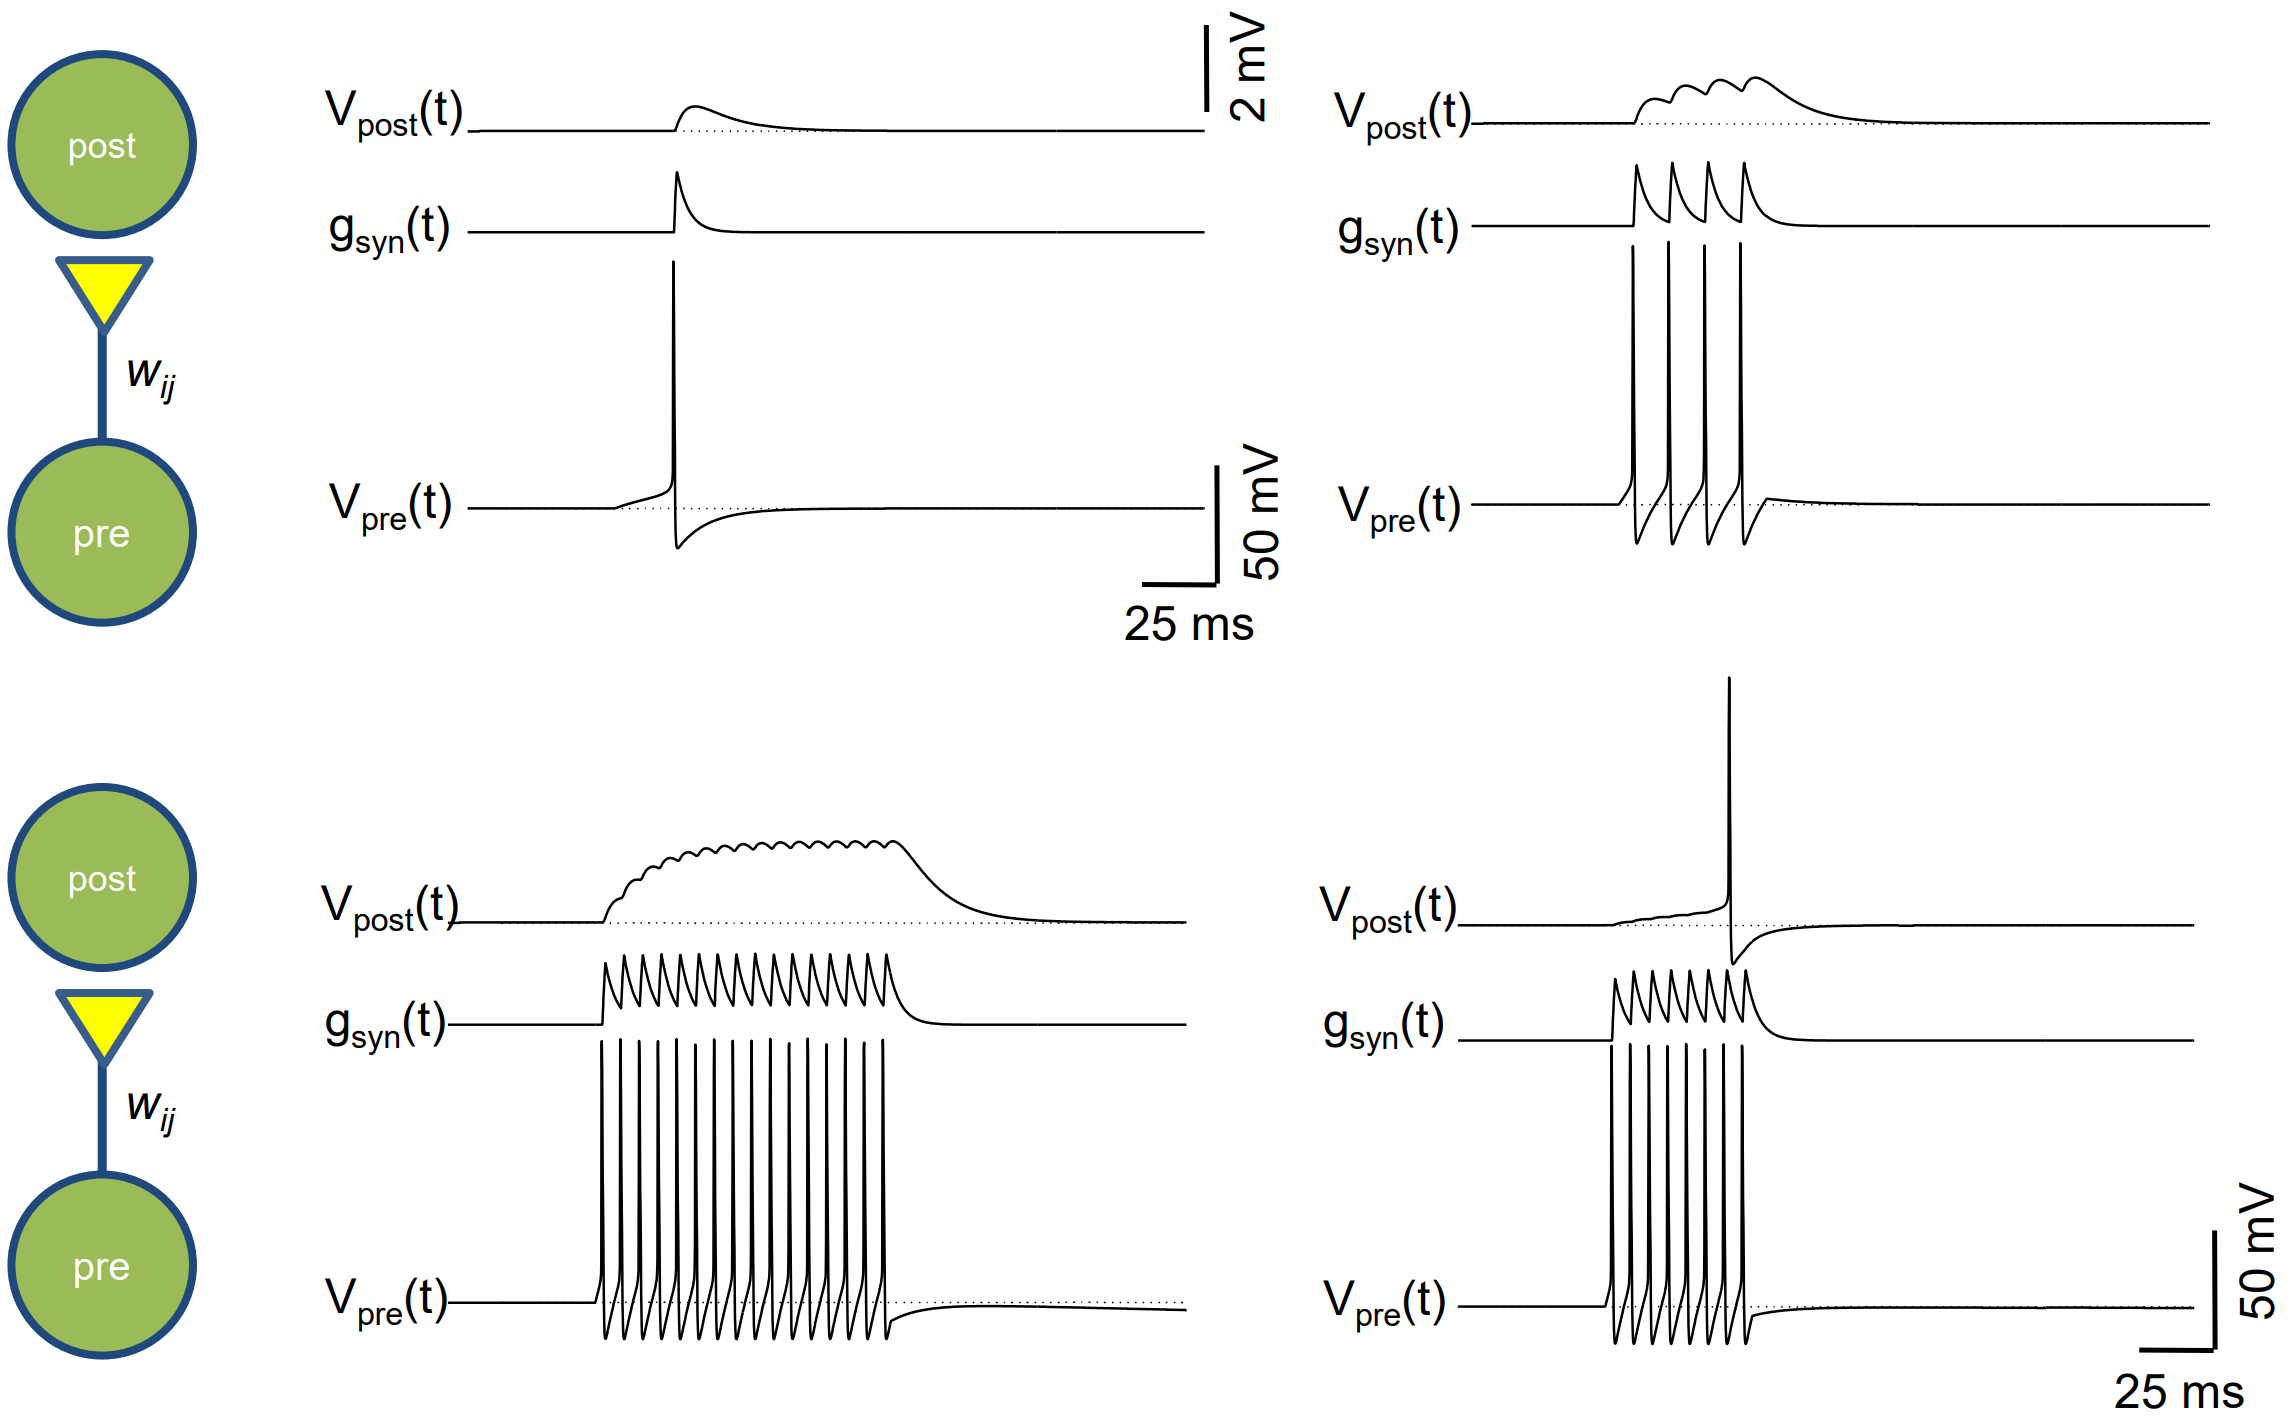
\includegraphics[scale=0.32]{12_5}
    \centering
\end{figure}
\subsubsection{Modelling Chemical Synapses}
When it comes to modelling chemical synapses, the idea is to use the typical
equivalent circuit for the postsynaptic neuron, but
a synaptic potential \(E_{syn}\) and conductance \(g_{syn}\) are to be added.
How to estimate such a conductance? The easiest case it to consider just two
states: open and close. An open synaptic channel will allow the flow of a fixed
amount of ions, hence will exhibit a fixed conductance. The synaptic current can be
computed as:
\begin{equation*}
    I_{syn}=g_{syn}(t)\bigl(V_{m}-E_{syn}\bigr)
\end{equation*}
Note that the postsynaptic conductance \(g_{syn}\) is driven by neurotransmitters
binding to ionotropic receptors, while the synaptic reversal potential \(E_{syn}\)
determines whether the synapse is excitatory or inhibitory.\\
Each synapse has number \(N\) of independent neurotransmitter release sites, thus
also the presynaptic neuron must be taken into account. Each of the \(N\) sites releases
nothing or a single synaptic vescicle, thus the release of neurotransmitters is
quantized by the number of vescicles. Hence, let's call \(P_{rel}\) the release
probability for each site, while \(N_{rel}\) is the average number of released vescicles:
\begin{equation*}
    N_{rel}=N\cdot{P_{rel}}
\end{equation*}
Finally, the synaptic current can be rewritten as:
\begin{equation*}
    I_{syn}=\bar{g}_{syn}\cdot{N_{rel}}\cdot{P_{rel}(t)}\cdot{\bigl(V_{m}-E_{syn}\bigr)}
\end{equation*}
where \(\bar{g}_{syn}\) is the maximum value for the synaptic conductance.\\
In the following, let's introduce some of the ways to model ionotropic
synapses, but first two important measures are to be defined:
Excitatory Post-Synaptic Current (EPSC) and Excitatory Post-Synaptic Potential (EPSP).
\paragraph{Instantaneous Rise + Single Exponential Decay}
This models aims at reproducing the behaviour of fast ionotropic synapses, where the
release of neurotransmitters and the opening of synaptic channels is assumed to be
instantaneous. As a matter of fact, the following is considered to be a good
model for AMPA receptors:
\begin{equation*}
    P_{rel}(t)=P_{max}\cdot{e^{-\frac{t-t_{0}}{\tau}}}
\end{equation*}
Note how the exponential term describes the decay of postsynaptic current, while
its rise occurs instantaneously.
\begin{figure}[H]
    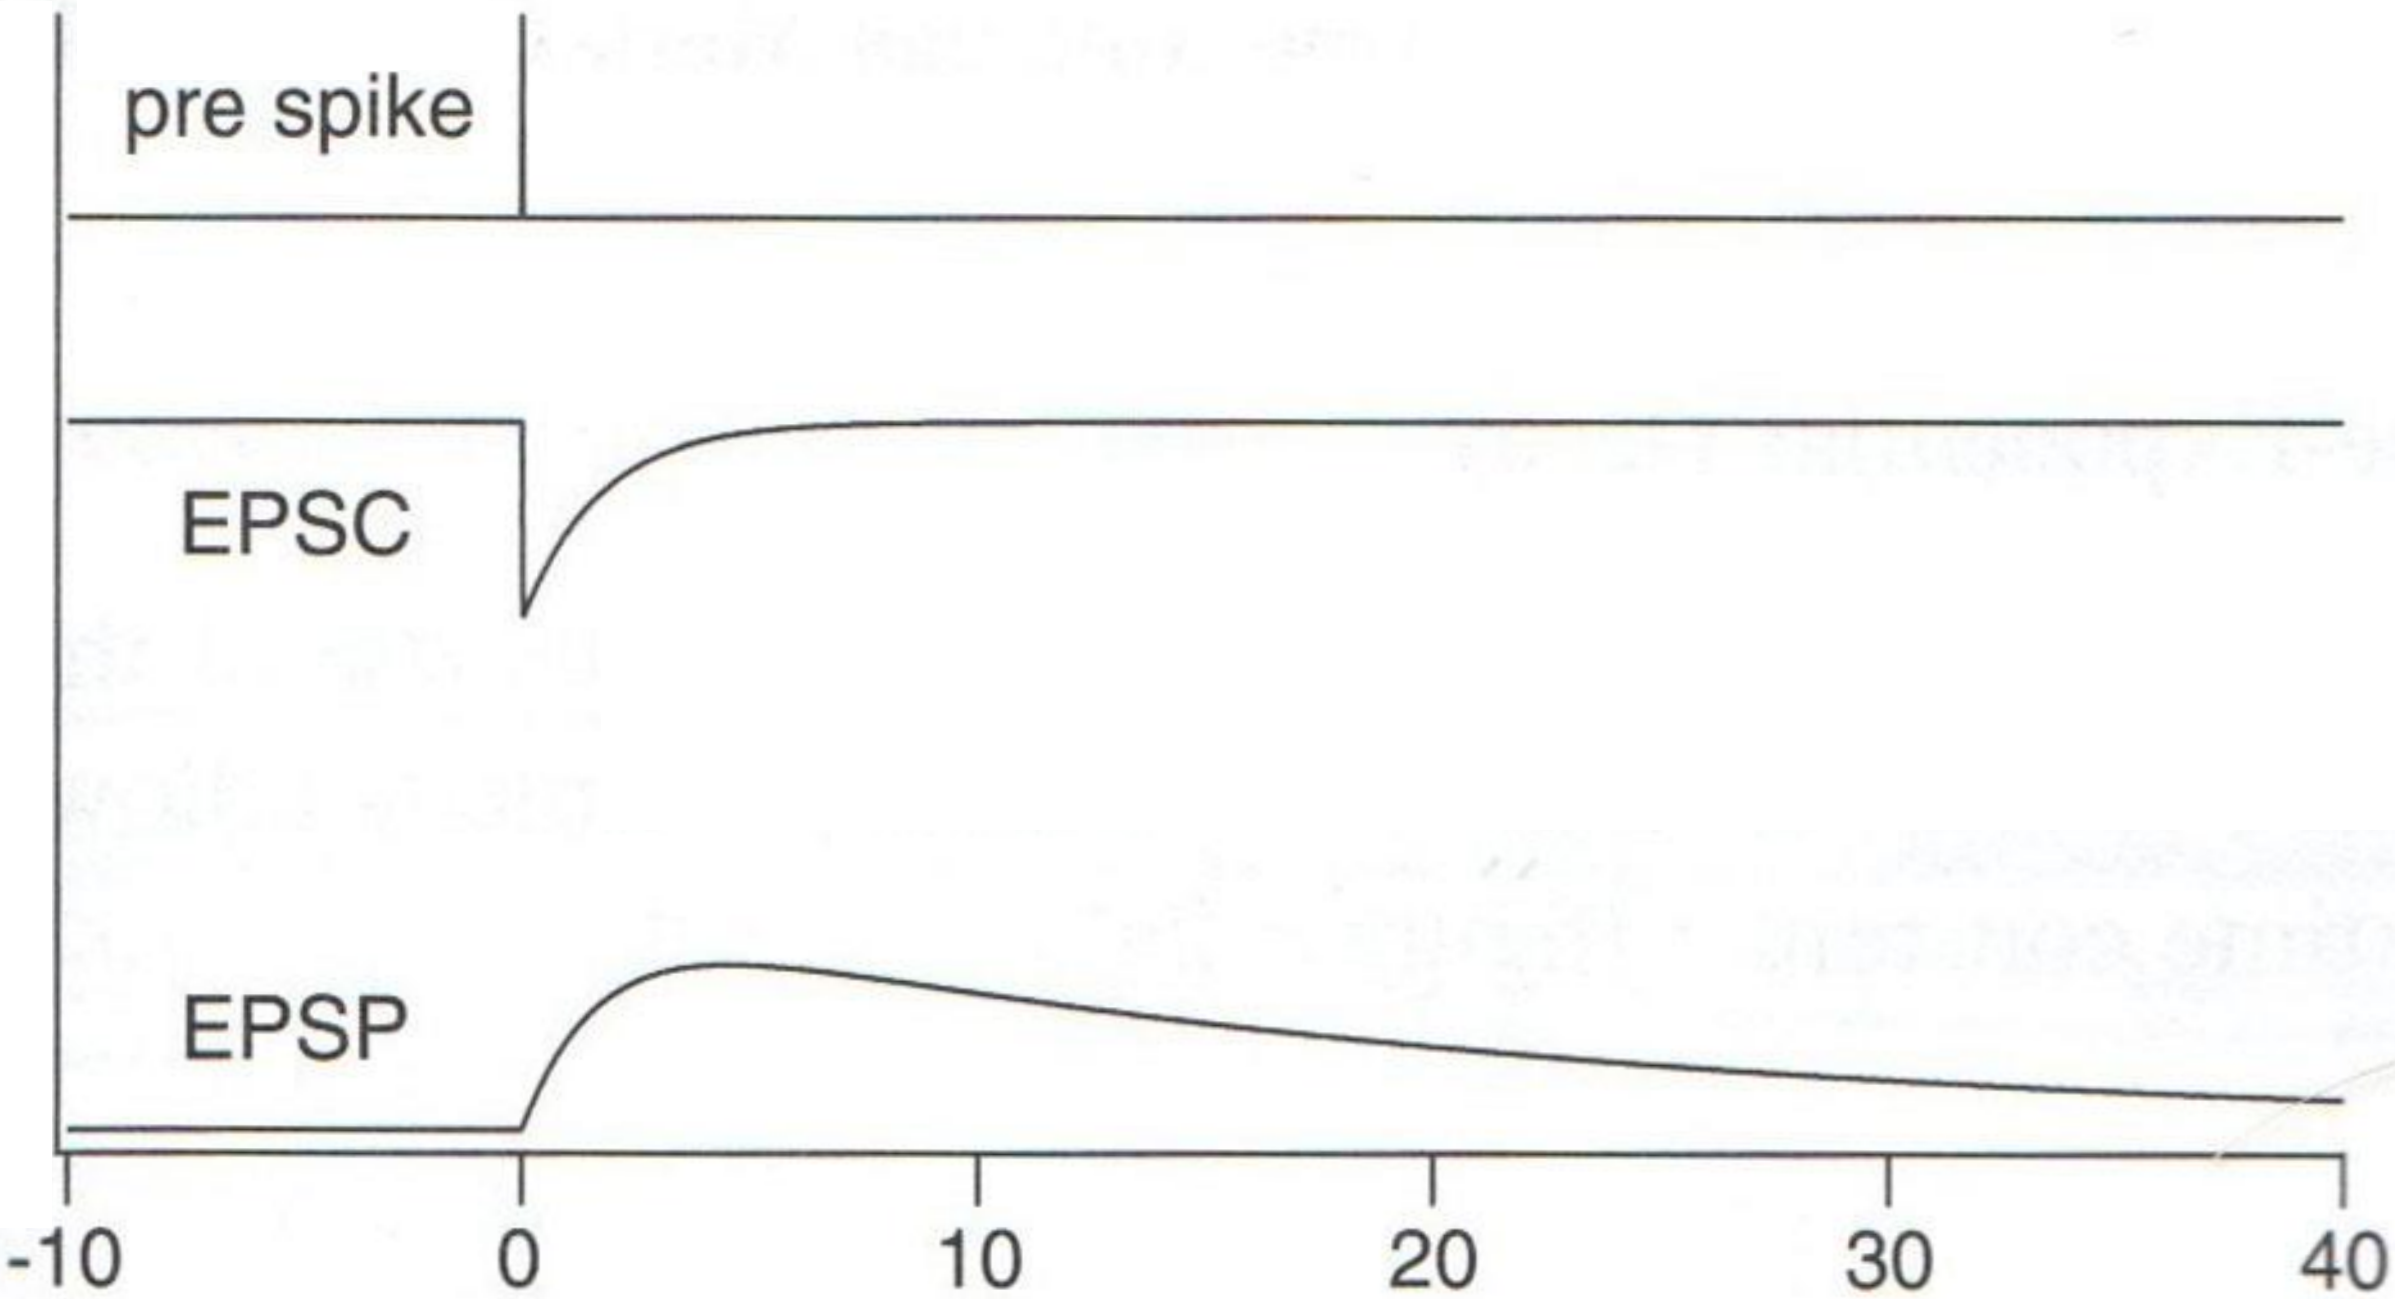
\includegraphics[scale=0.2]{12_6}
    \centering
\end{figure}
\paragraph{Alpha Function}
In this case the release probability kernel function is substituted by an alpha function,
which substitutes the sharp depolarization and current rise with a smoother curve.
\begin{equation*}
    P_{rel}(t)=P_{max}\cdot\frac{t-t_{0}}{\tau}\cdot{e^{-\frac{t-t_{0}}{\tau}}}
\end{equation*}
Note that only one time constant \(\tau\) is employed, settings a relationship
between the rise and decay dynamics of the EPSC. This won't allow to set them
independently and it is not realistic from a physiological viewpoint.
\begin{figure}[H]
    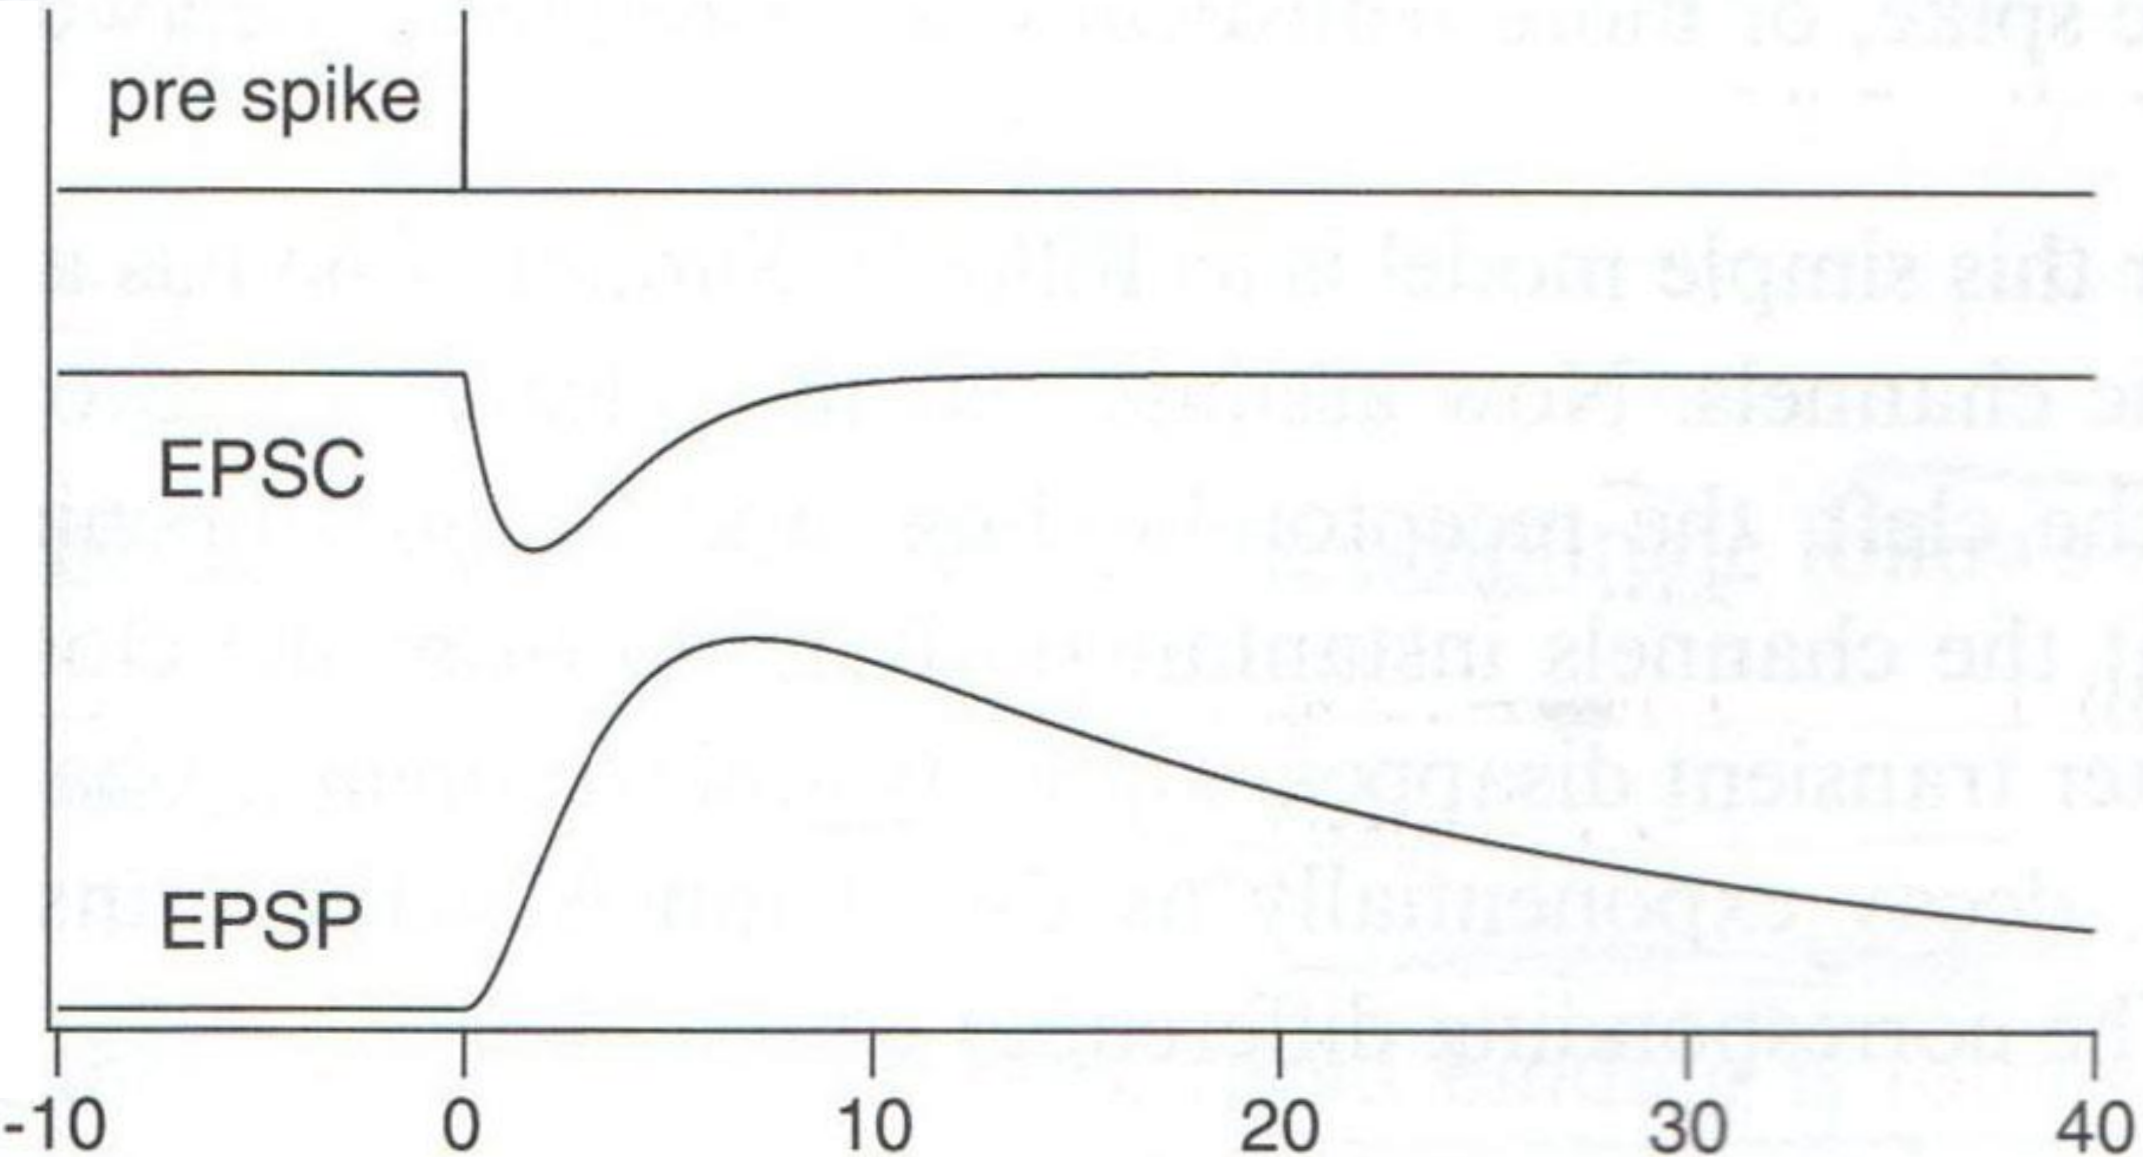
\includegraphics[scale=0.22]{12_7}
    \centering
\end{figure}
\paragraph{Difference of Two Exponentials}
Lastly, this model tries to overcome the limitation imposed by the alpha function
by introducing two independent time constants, regulating the rise and
decay of EPSC in an uncoupled way.
\begin{equation*}
    P_{rel}(t)=P_{max}\Bigl(e^{-\frac{t-t_{0}}{\tau_{decay}}}-e^{-\frac{t-t_{0}}{\tau_{rise}}}\Bigr)
\end{equation*}
\begin{figure}[H]
    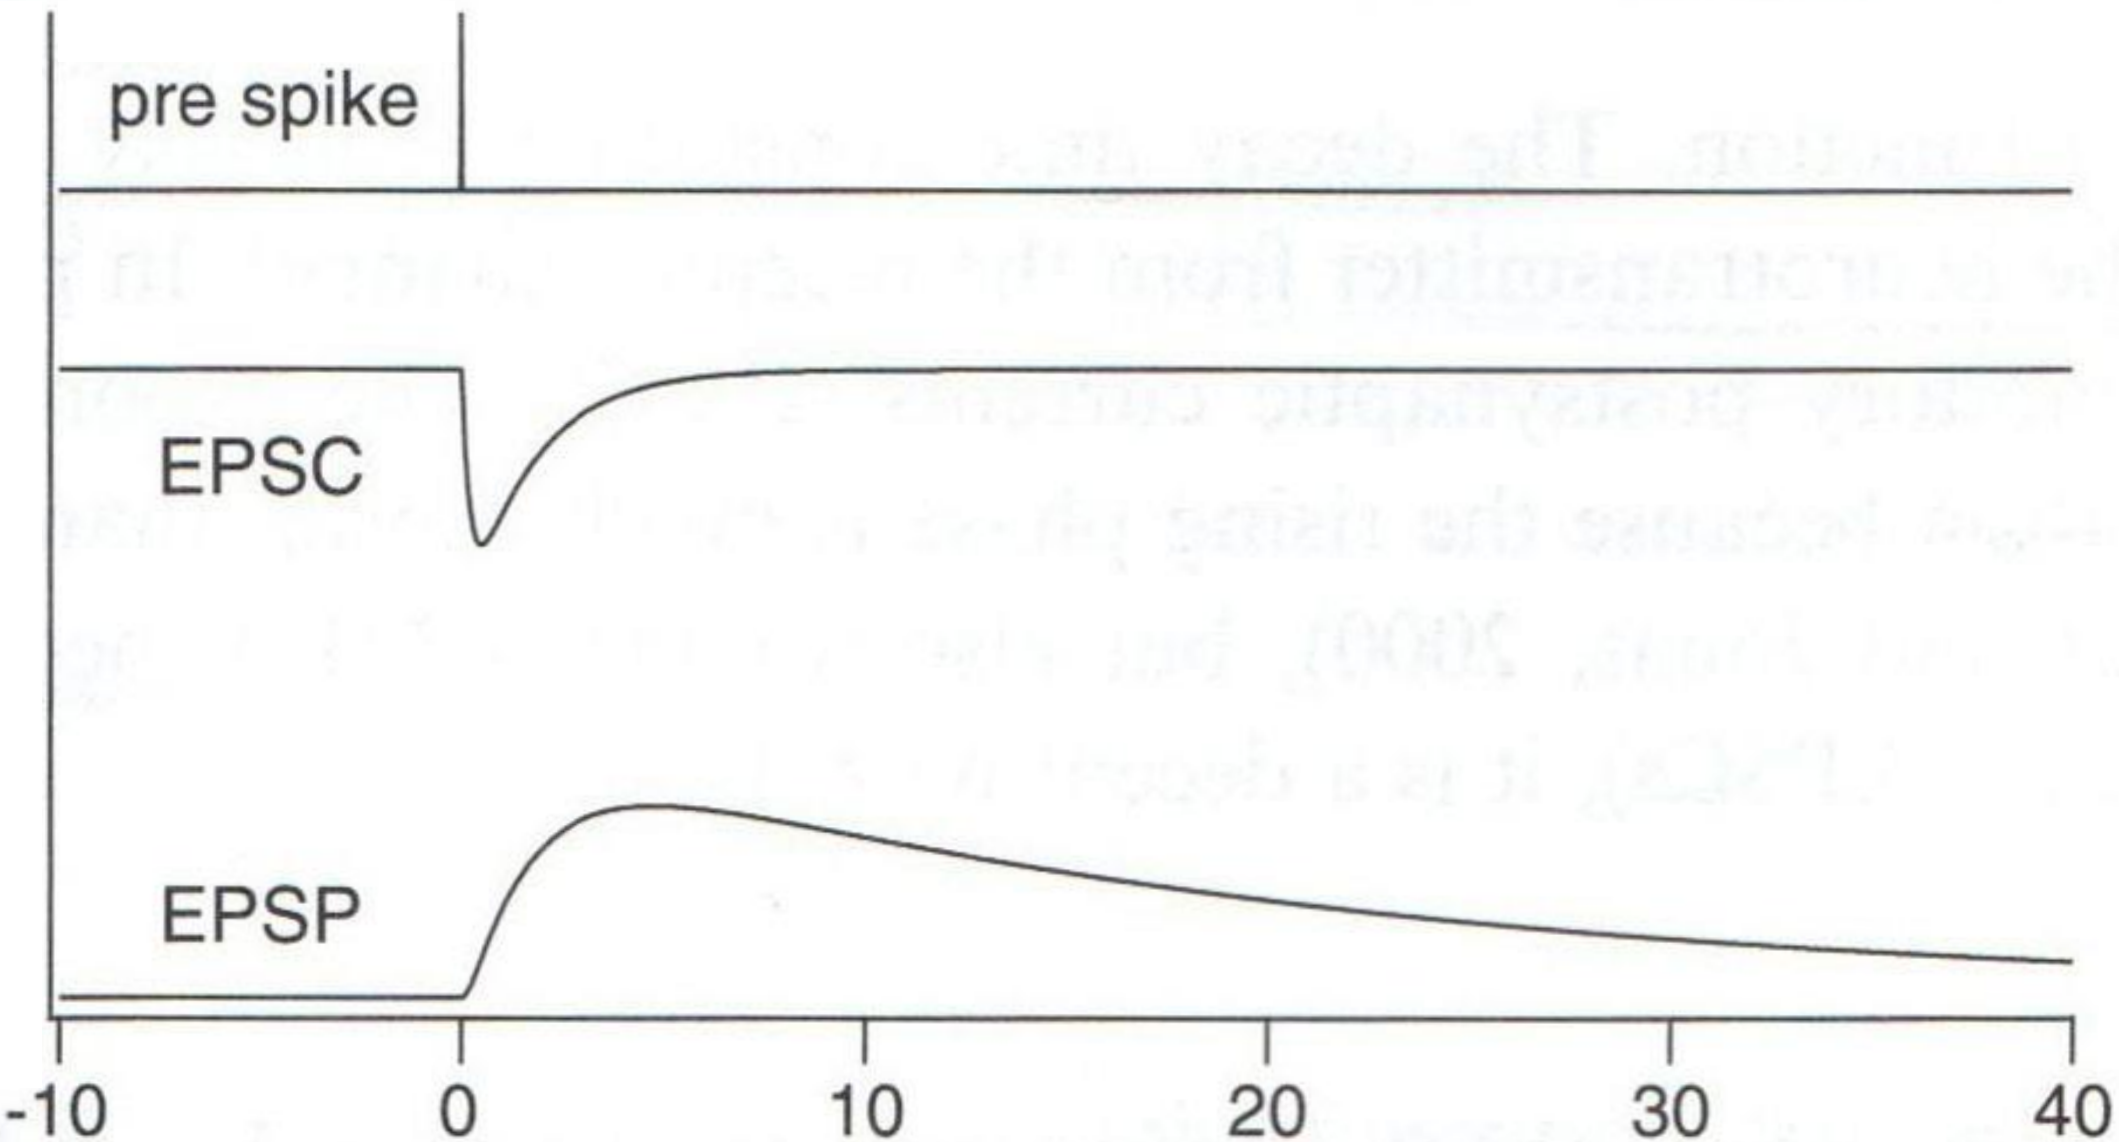
\includegraphics[scale=0.22]{12_8}
    \centering
\end{figure}
\textbf{CAPIRE \(\tau_{peak}\) e \(f\): VEDERE GRAFICI DESMOS!}
\par
As stated before, different models can be used to represent the behaviour of different types of
neurotransmitters receptors, as illustrated in the figure below.
\begin{figure}[H]
    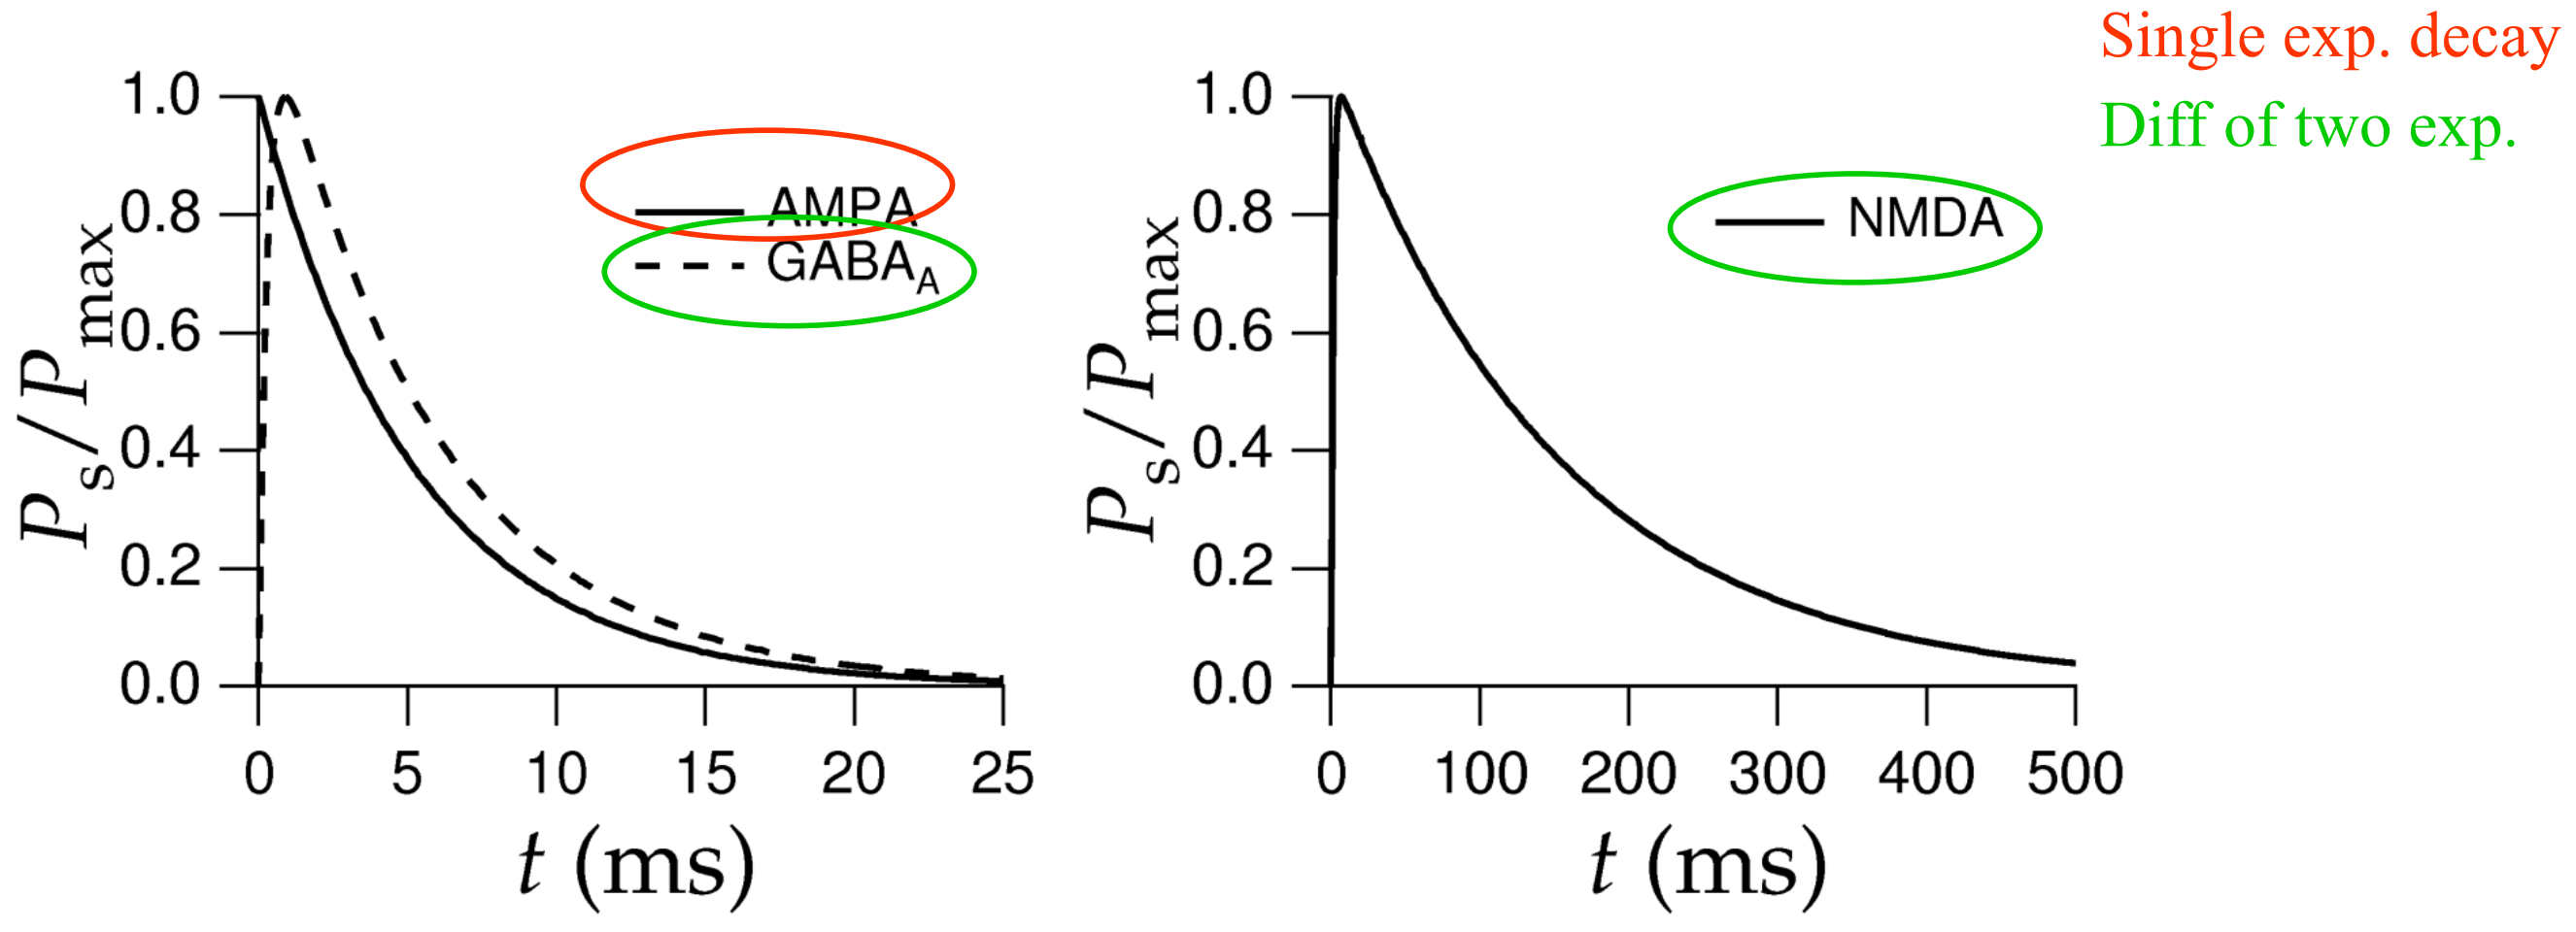
\includegraphics[scale=0.25]{12_9}
    \centering
\end{figure}
Henceforth, the full model of a ionotropic postsynaptic neuron by the phenomenological
approach can be written as:
\begin{equation*}
    I_{syn}=\bar{g}_{syn}\cdot{N_{rel}}\cdot{P_{rel}(t)}\cdot{(V_{m}-E_{syn})}
    \hspace{1.15cm}
    \text{where}
    \hspace{0.15cm}
    P_{rel}(t)=
    \begin{cases}
        P_{max}\cdot{e^{-\frac{t-t_{0}}{\tau}}}\\
        P_{max}\cdot\frac{t-t_{0}}{\tau}\cdot{e^{-\frac{t-t_{0}}{\tau}}}\\
        P_{max}\cdot{f}\cdot\Bigl(e^{-\frac{t-t_{0}}{\tau_{decay}}}-e^{-\frac{t-t_{0}}{\tau_{rise}}}\Bigr)
    \end{cases}
\end{equation*}
Note that the synaptic weight is represented by
\(
    w=\bar{g}_{syn}\cdot{N_{rel}}\cdot{P_{rel}(t)}
\)
leading to:
\begin{equation*}
    I_{syn}=w\cdot{(V_{m}-E_{syn})}
\end{equation*}
If plasticity is to be taken into account, this can be considered in the modelling of the
release probability \(P_{rel}(t)\), which can be increased (potentiation) or decreased
(depression). This will affect the synaptic weight \(w\), which can be either
time-dependent or time-invariant.
\subsubsection{Alternative Synaptic Modelling}
\paragraph{Conductance-based (COBA) Model}
The COBA synaptic model takes into account both excitatory and inhibitory synapses:
\begin{equation*}
    I_{syn}=g_{syn}^{e}(V_{m}-E_{syn}^{e})+g_{syn}^{i}(V_{m}-E_{syn}^{i})
\end{equation*}
Now, let's plug this cumulative synaptic current into the LIF model, obtaining a
COBA LIF neuron model:
\begin{equation*}
    C_{m}\frac{dV_{m}}{dt}=g_{leak}(V_{m}-E_{leak})+g_{syn}^{e}(V_{m}-E_{syn}^{e})+g_{syn}^{i}(V_{m}-E_{syn}^{i})+I_{stim}
\end{equation*}
Note that \(I_{syn}=I_{syn}(t)\) is time-varying, as the conductances are not time-invariant. Therefore,
the relationship between \(V_{m}\) and its derivative is no longer time-invariant, as it depends also
on synaptic conductances. Moreover, the summation of postsynaptic potentials (PSPs) is no longer
linear and the total membrane conductance \(g_{tot}=g_{leak}+g_{syn}^{e}+g_{syn}^{i}\) is itself
a function of time and results larger than \(g_{leak}\) itself, as conductances are
always positive.\\
The reaction speed of the membrane is now time-dependent and described
by its time constant:
\begin{equation*}
    \tau_{eff}=\frac{C_{m}}{g_{tot}}
\end{equation*}
This means that the effect on the membrane potential of an incoming spike depends on
all the other spikes received from all the presynaptic partners.\\
At this point, let's consider a generic synaptic conductance (either excitatory or inhibitory)
modelled by an exponential kernel. It can be written as:
\begin{equation*}
    g_{syn}^{x}(t)=\sum_{k}^{synapses}\sum_{s}^{spikes}P_{max}^{k}\theta{(t-t_{s})}e^{-\frac{t-t_{s}}{\tau_{syn}}}
\end{equation*}
Thus, the synaptic conductance is activated only whenever there is a spike triggering
the synapse. Finally, the total synaptic current is given by:
\begin{equation*}
    I_{syn}(t,V_{m})=\sum_{x\in{\{e,i\}}}\sum_{k}^{synapses}\sum_{s}^{spikes}P_{max}^{k}\theta{(t-t_{s})}(V_{m}-E_{syn}^{x})e^{-\frac{t-t_{s}}{\tau_{syn}}}
\end{equation*}
\paragraph{Current-based (CUBA) Model}
An incoming spike may cause a local variation in the membrane conductance, but the
elicited postsynaptic potential (PSP) propagates passively towards the soma,
which acts as an integrator centre, where all the inputs are summed up
to eventually generate action potentials. Hence, a COBA model
should be combined with a point neuron model, which approximate the soma:
\begin{equation*}
    C_{m}\frac{dV_{m}}{dt}=g_{leak}(V_{m}-E_{leak})+I_{syn}+I_{ext}
\end{equation*}
where the synaptic current is time-dependent and defined as:
\begin{equation*}
    I_{syn}(t)=\sum_{k}^{synapses}\sum_{s}^{spikes}P_{max}^{k}\theta{(t-t_{s})}e^{-\frac{t-t_{s}}{\tau_{syn}}}
\end{equation*}
Note that PSPs in the CUBA model are integrated linearly, without
interacting with each other.
\pagebreak
If COBA and CUBA models are to be compared, it can be seen that the
signals are almost equivalent. It can be observed a PSP
saturation, stronger in the COBA model, as the membrane
potential approaches the reversal potential. Another thing to observe
is that when stimulated by an identical Poissonian spike train,
the CUBA neuron membrane potential fluctuates significantly
stronger than the one of the COBA model, as the CUBA neuron
total conductance is lower with respect to the COBA one,
leading to a slower membrane dynamics and therefore larger PSPs.
\begin{figure}[H]
    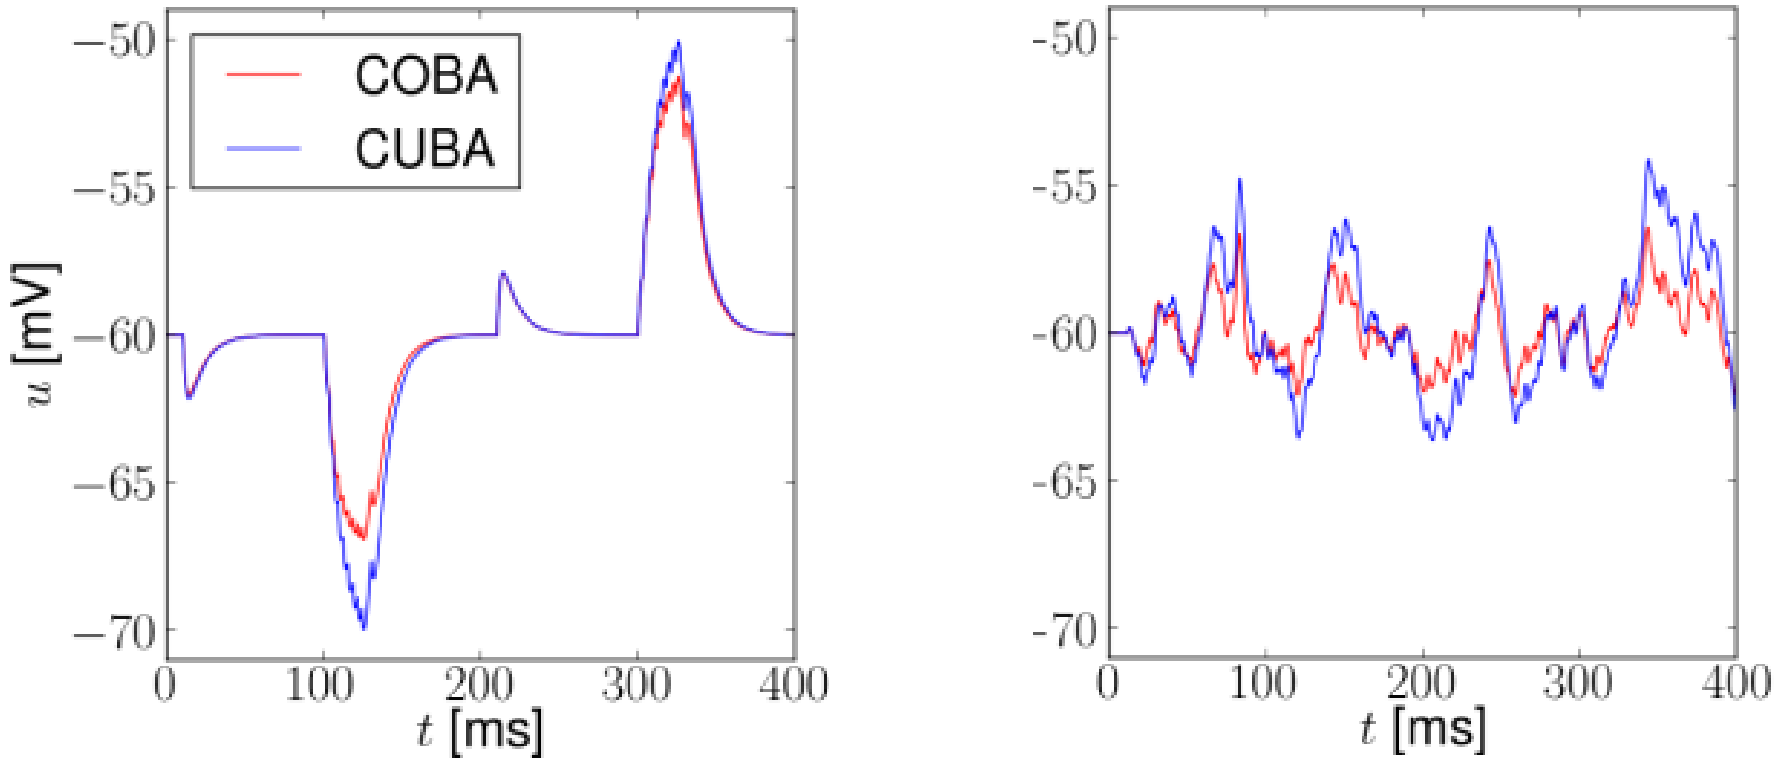
\includegraphics[scale=0.35]{12_10}
    \centering
\end{figure}
A significant difference between the two models can be observed whenever the
inputs are integrated. The CUBA model tends to show much less bursting activity,
while the COBA neuron activity is characterized by bursts.
\begin{figure}[H]
    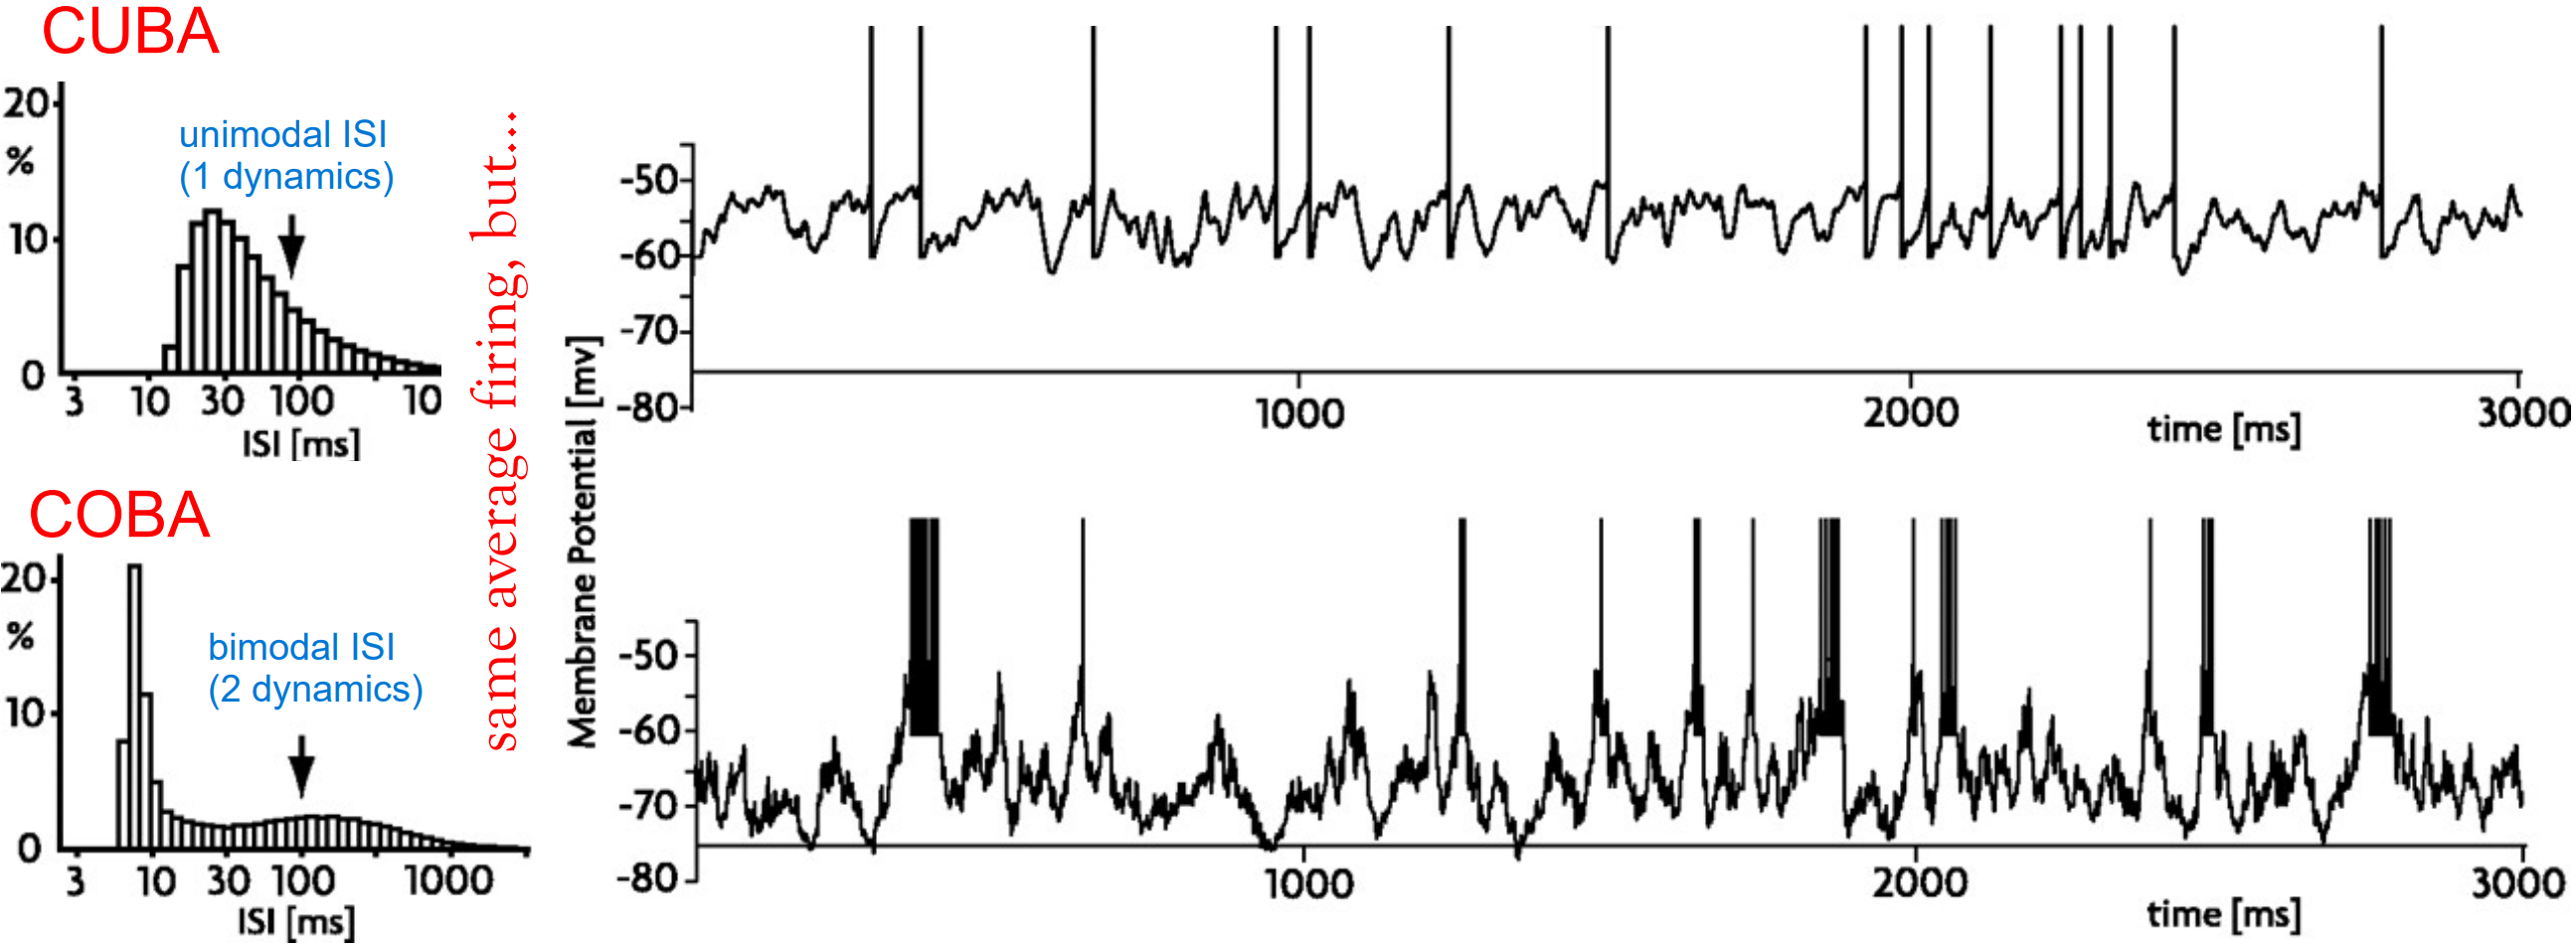
\includegraphics[scale=0.3]{12_11}
    \centering
\end{figure}